\documentclass{beamer}
\usepackage[utf8]{inputenc}

\usetheme{Madrid}
\usecolortheme{default}
\usepackage{amsmath,amssymb,amsfonts,amsthm}
\usepackage{txfonts}
\usepackage{tkz-euclide}
\usepackage{listings}
\usepackage{adjustbox}
\usepackage{array}
\usepackage{tabularx}
\usepackage{gvv}
\usepackage{lmodern}
\usepackage{circuitikz}
\usepackage{tikz}
\usepackage{graphicx}
\usepackage{multicol}
\setbeamertemplate{page number in head/foot}[totalframenumber]

\usepackage{tcolorbox}
\tcbuselibrary{minted,breakable,xparse,skins}



\definecolor{bg}{gray}{0.95}
\DeclareTCBListing{mintedbox}{O{}m!O{}}{%
  breakable=true,
  listing engine=minted,
  listing only,
  minted language=#2,
  minted style=default,
  minted options={%
    linenos,
    gobble=0,
    breaklines=true,
    breakafter=,,
    fontsize=\small,
    numbersep=8pt,
    #1},
  boxsep=0pt,
  left skip=0pt,
  right skip=0pt,
  left=25pt,
  right=0pt,
  top=3pt,
  bottom=3pt,
  arc=5pt,
  leftrule=0pt,
  rightrule=0pt,
  bottomrule=2pt,

  colback=bg,
  colframe=orange!70,
  enhanced,
  overlay={%
    \begin{tcbclipinterior}
    \fill[orange!20!white] (frame.south west) rectangle ([xshift=20pt]frame.north west);
    \end{tcbclipinterior}},
  #3,
}
\lstset{
    language=C,
    basicstyle=\ttfamily\small,
    keywordstyle=\color{blue},
    stringstyle=\color{orange},
    commentstyle=\color{green!60!black},
    numbers=left,
    numberstyle=\tiny\color{gray},
    breaklines=true,
    showstringspaces=false,
}
%------------------------------------------------------------
%This block of code defines the information to appear in the
%Title page
\title %optional
{4.2.15}
\date{September  2025}
%\subtitle{A short story}

\author % (optional)
{BEERAM MADHURI - EE25BTECH11012}



\begin{document}


\frame{\titlepage}
\begin{frame}{Question}
Three distinct points $A$, $B$ and $C$ are given in the 2-dimensional coordinate plane such that the ratio of the distance of any one of them from the point $(1,0)$ to the distance from the point $(-1,0)$ is equal to $\frac{1}{3}$. Then the circumcentre of the triangle $ABC$ is at the point:
\begin{enumerate}
\begin{multicols}{4}
\item $\left(\frac{5}{4}, 0\right)$
\item $\left(\frac{5}{2}, 0\right)$
\item $\left(\frac{5}{3}, 0\right)$
\item $(0, 0)$
\end{multicols}
\end{enumerate}
\end{frame}
 
\begin{frame}{given data}
 let $\vec{F_1}$, $\vec{F_2}$ be the vectors such that:
\begin{table}[h!]
    \centering
    \begin{tabular}[12pt]{ |c| c|}
    \hline
    \textbf{Point} & \textbf{Vector}\\ 
    \hline
    $\mathbf{v_1}$ &  $\myvec{1\\1\\1}$\\
    \hline
    $\mathbf{v_2}$ &   $\myvec{1\\-1\\1}$\\
    \hline
     $\mathbf{v_3}$ &  $\myvec{1\\1\\-1}$\\
    \hline
    \end{tabular}
    \caption{Variables used}
    \label{table 1.9.1}
\end{table}
\end{frame}

\begin{frame}{solution}
    \frametitle{finding the Circumcenter of the triangle formed by A,B and C}
Let $\vec{P}$ be any vector in the plane of $\vec{A}$,$\vec{B}$,$\vec{C}$.\\
  given,
\begin{align}
\frac{\| \vec{PF_1} \|}{\| \vec{PF_2} \|} = \frac{1}{3}\\
\frac{\sqrt{(\vec{P}-\vec{F_1})^\top (\vec{P}-\vec{F_1})}}{\sqrt{(\vec{P}-\vec{F_2})^\top (\vec{P}-\vec{F_2})}} = \frac{1}{3}
\end{align}
\end{frame}
\begin{frame}
Squaring on both sides
\begin{align}
9 (\vec{P}-\vec{F_1})^\top (\vec{P}-\vec{F_1}) = (\vec{P}-\vec{F_2})^\top (\vec{P}-\vec{F_2})\\
9 (\vec{P^\top} \vec{P} - \vec{P^\top} \vec{F_1} - \vec{F_1^\top} \vec{P} + \vec{F_1^\top} \vec{F_1}) = \vec{P^\top} \vec{P} - \vec{P^\top} \vec{F_2} - \vec{F_2^\top} \vec{P} + \vec{F_2^\top} \vec{F_2}
\end{align}
\begin{align}
\text{as } \vec{P^\top} \vec{F_1} = \vec{F_1}^\top \vec{P} \\
\text{and } \vec{P^\top} \vec{F_2} = \vec{F_2^\top} \vec{P}
\end{align}
\begin{align}
9 (\vec{P^\top} \vec{P} - 2\vec{P^\top} \vec{F_1} + \vec{F_1^\top} \vec{F_1}) = \vec{P^\top} \vec{P} - 2\vec{P^\top} \vec{F_2} + \vec{F_2^\top} \vec{F_2}\\
8 \vec{P^\top} \vec{P} - 2\vec{P^\top} (9\vec{F_1}-\vec{F_2}) +9\vec{F_1^\top} \vec{F_1} - \vec{F_2^\top} \vec{F_2} = 0\\
\vec{P^\top} \vec{P} - \frac{1}{4} \vec{P^\top} (9\vec{F_1}-\vec{F_2}) + \frac{9}{8} \vec{F_1^\top} \vec{F_1} - \frac{1}{8} \vec{F_2^\top} \vec{F_2} = 0
\end{align}
\end{frame}
\begin{frame}
This can be compared with general equation of circle :
\begin{align}
||\vec{P} - \vec{C}|| = r\\
\end{align}
\text{
where ,}
\text{
$\vec{P}$ = any point on the circle}\\
\text{$\vec{C}$ = Center of circle}\\
\text{
r = radius of circle}
\end{frame}
\begin{frame}
\begin{align}
(\vec{P}-\vec{C})^\top(\vec{P}-\vec{C}) = r^2\\
\vec{P}^\top\vec{P} -2\vec{P}^\top\vec{C}+\vec{C}^\top\vec{C}=r^2
\end{align}
Substituting $\Vec{P}$, $\vec{F_1}$ and $\vec{F_2}$\\
Center of circle =  $\left(\frac{5}{4}, 0\right)$

Hence, the circumcenter of the triangle is $\left(\frac{5}{4}, 0\right)$
\end{frame}


\begin{frame}[fragile]
    \frametitle{Python Code}
    \begin{lstlisting}
import matplotlib.pyplot as plt
import numpy as np

# --- 1. Define the geometric elements ---

# The two fixed points from the problem
f1 = np.array([1, 0])
f2 = np.array([-1, 0])
\end{lstlisting}
\end{frame}

\begin{frame}[fragile]
\frametitle{Python Code}
\begin{lstlisting}
# The locus of points P such that dist(P, F1) / dist(P, F2) = 1/3 is a circle.
# By solving the distance equation, we find the circle's properties:
# 9 * ((x-1)^2 + y^2) = (x+1)^2 + y^2
# 8x^2 - 20x + 8y^2 + 8 = 0
# x^2 - (5/2)x + y^2 + 1 = 0
# (x - 5/4)^2 + y^2 = (3/4)^2
# The center of this circle is the circumcenter of triangle ABC.
circumcenter = np.array([5/4, 0])
radius = 3/4
\end{lstlisting}
\end{frame}

\begin{frame}[fragile]
\frametitle{Python Code}
\begin{lstlisting}
theta = np.linspace(0, 2 * np.pi, 200)
circle_x = circumcenter[0] + radius * np.cos(theta)
circle_y = circumcenter[1] + radius * np.sin(theta)
angles = np.array([np.pi/4, 5*np.pi/6, 3*np.pi/2])
A = circumcenter + radius * np.array([np.cos(angles[0]), np.sin(angles[0])])
B = circumcenter + radius * np.array([np.cos(angles[1]), np.sin(angles[1])])
C = circumcenter + radius * np.array([np.cos(angles[2]), np.sin(angles[2])])
triangle_points = np.array([A, B, C, A]) # Add A at the end to close the triangle
\end{lstlisting}
\end{frame}

\begin{frame}[fragile]
\frametitle{Python Code}
\begin{lstlisting}
# --- 3. Create the plot ---

# Set up the plot style and figure
plt.style.use('seaborn-v0_8-whitegrid')
fig, ax = plt.subplots(figsize=(10, 8))

# Plot the circumcircle
ax.plot(circle_x, circle_y, 'b-', label='Locus of A, B, C (Circumcircle)')

\end{lstlisting}
\end{frame}

\begin{frame}[fragile]
\frametitle{Python Code}
\begin{lstlisting}
# Plot the example triangle ABC
ax.plot(triangle_points[:, 0], triangle_points[:, 1], 'g--', marker='o', markersize=8, label='Example Triangle ABC')
# Plot the two fixed points
ax.plot(f1[0], f1[1], 'ro', markersize=10, label='Fixed Point F1 (1, 0)')
ax.plot(f2[0], f2[1], 'mo', markersize=10, label='Fixed Point F2 (-1, 0)')
# Plot and highlight the circumcenter
ax.plot(circumcenter[0], circumcenter[1], 'k*', markersize=15, label=f'Circumcenter ({circumcenter[0]}, {circumcenter[1]})')
\end{lstlisting}
\end{frame}

\begin{frame}[fragile]
\frametitle{Python Code}
\begin{lstlisting}

# --- 4. Add labels and formatting ---

# Annotate the points on the graph
ax.text(A[0], A[1] + 0.1, 'A', fontsize=14, color='green')
ax.text(B[0] - 0.15, B[1], 'B', fontsize=14, color='green')
ax.text(C[0], C[1] - 0.15, 'C', fontsize=14, color='green')
ax.text(circumcenter[0], circumcenter[1] + 0.05, 'Circumcenter', fontsize=12, ha='center')

\end{lstlisting}
\end{frame}

\begin{frame}[fragile]
\frametitle{Python Code}
\begin{lstlisting}

# Set plot title and axis labels
ax.set_title('Solution for Finding the Circumcenter', fontsize=16)
ax.set_xlabel('X-axis', fontsize=12)
ax.set_ylabel('Y-axis', fontsize=12)

# Ensure the aspect ratio is equal to prevent the circle from looking like an ellipse
ax.set_aspect('equal', adjustable='box')
ax.axhline(0, color='black', linewidth=0.5)
ax.axvline(0, color='black', linewidth=0.5)
\end{lstlisting}
\end{frame}

\begin{frame}[fragile]
\frametitle{Python Code}
\begin{lstlisting}
# Add legend and grid
ax.legend(loc='upper right')
ax.grid(True)

# Set axis limits for a clean view
ax.set_xlim(-2, 3)
ax.set_ylim(-1.5, 1.5)

# Display the final plot
plt.show()
\end{lstlisting}
\end{frame}

\begin{frame}[fragile]
\frametitle{C Code}
\begin{lstlisting}
#include <stdio.h>
#include <math.h>

struct Point {
    double x;
    double y;
};
struct Point findCircumcenter(struct Point p1, struct Point p2, double ratio) {
    struct Point center;
    double k = ratio;
    double k_squared = k * k;
\end{lstlisting}
\end{frame}

\begin{frame}[fragile]
\frametitle{C Code}
\begin{lstlisting}
// Formula for the center of the Circle of Apollonius
// Center (h, k) = ( (x1 - k^2*x2) / (1 - k^2), (y1 - k^2*y2) / (1 - k^2) )
center.x = (p1.x - k_squared * p2.x) / (1 - k_squared);
center.y = (p1.y - k_squared * p2.y) / (1 - k_squared);
return center;
}

int main() {
// Define the two fixed points from the problem
struct Point p1 = {1.0, 0.0};  // Point (1, 0)
struct Point p2 = {-1.0, 0.0}; // Point (-1, 0)
\end{lstlisting}
\end{frame}

\begin{frame}[fragile]
\frametitle{C Code}
\begin{lstlisting}
// Define the given ratio
double ratio = 1.0 / 3.0;

// Calculate the circumcenter
struct Point circumcenter = findCircumcenter(p1, p2, ratio);
printf("The circumcenter of the triangle ABC is at the point: (%.2f, %.2f)\n",
circumcenter.x, circumcenter.y);
printf("In fraction form, this is (5/4, 0).\n");
return 0;
}
\end{lstlisting}
\end{frame}

\begin{frame}[fragile]
\frametitle{Python and C Code}
\begin{lstlisting}
import ctypes

# Define a structure equivalent to C struct Point
class Point(ctypes.Structure):
    _fields_ = [("x", ctypes.c_double),
                ("y", ctypes.c_double)]

def find_circumcenter(p1: Point, p2: Point, ratio: float) -> Point:
    center = Point()
    k = ratio
    k_squared = k * k
\end{lstlisting}
\end{frame}

\begin{frame}[fragile]
\frametitle{Python and C Code}
\begin{lstlisting}
    # Apply the same formula as in the C code
    center.x = (p1.x - k_squared * p2.x) / (1 - k_squared)
    center.y = (p1.y - k_squared * p2.y) / (1 - k_squared)
    return center
if __name__ == "__main__":
    # Define the two points
    p1 = Point(1.0, 0.0)
    p2 = Point(-1.0, 0.0)
\end{lstlisting}
\end{frame}

\begin{frame}[fragile]
\frametitle{Python and C Code}
\begin{lstlisting}
    # Define the ratio
    ratio = 1.0 / 3.0

    # Compute the circumcenter
    circumcenter = find_circumcenter(p1, p2, ratio)

    # Print the result
    print(f"The circumcenter of the triangle ABC is at the point: ({circumcenter.x:.2f}, {circumcenter.y:.2f})")
    print("In fraction form, this is (5/4, 0).")

\end{lstlisting}
\end{frame}
\begin{frame}
\begin{figure}
    \centering
    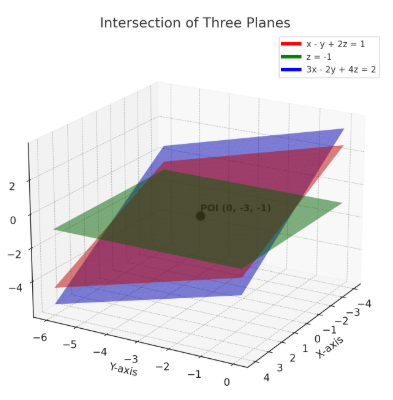
\includegraphics[width=0.75\columnwidth]{graph9.png}
    \caption{Plot}
    \label{fig:placeholder}
\end{figure}
\end{frame}

\end{document}